\chapter{IMPLEMENTATION}
\paragraph\
This chapter gives a brief description of the implementation details of the testing plan and obstacles faced during implementation.

\section {The test plan}
The initial step was to test the services with \acs{IPVS} thesis publications \cite{thesispublications} dataset to get an idea of how the services can be used. This was chosen as the thesis dataset already had the concised or an overview version available to view the abstract, author, and supervisor fields for each thesis file. It would be easy to validate and understand the features with an already labeled dataset. An example of the thesis file \ref{sampledatadetail} and a summarized version \ref{sampledataconcise} available in \cite{thesispublications} can be seen in the Appendix section. The next phase was the actual testing to evaluate the service and fill in the evaluation matrix. The plan includes performing the testing of the services on three different datasets for various parameters listed. Each dataset was tested two times to confirm the consistency in results. 

\section {Implementation}  %IN progress
\label{section:impl}
As obtaining access to Microsoft Azure was relatively easy, testing was started with Microsoft Azure Cognitive Search Services \cite{azdocs} after completing the initial tutorial lab as part of the Microsoft Learn training module \cite{azuretutorial}.
Below is a step-by-step implementation done in Microsoft Azure with screenshots from the testing done on sample test data (\acs{IPVS} thesis data set \cite{thesispublications}):
\begin{itemize}
    \item Created a resource 'Azure Cognitive Search' named \textit{searchservicesampledata}.
    \item Created a resource group to add the resources to \textit{rg\_sampledata}.
    \item Created a resource 'Cognitive Services' named \textit{cogservicesampledata}.
    \item Created a resource 'Storage Account' named \textit{sampledatastrgacc}. A snapshot of Azure resources created can be seen in Appendix \ref{azureresources}.
    \item Created a container in the storage account and uploaded the sample dataset in it.
    \item Imported the dataset in Azure Cognitive Search resource (\textit{searchservicesampledata}) and created and Index following the steps below:
    \begin{itemize}
        \item First step was 'Connect to your data'. Connected storage account to Cognitive search resource and selected the dataset uploaded in a storage account.
        \item Next step was 'Add Cognitive skills'. 
        In this tab, there were 3 sections; 
        \begin{enumerate}
            \item First section was the 'Attach Cognitive Services' section. In this section, the dataset was attached to created cognitive services resource (\textit{cogservicesampledata}).
            \item Second section was 'Add enrichments'. In this, choosing and setting up cognitive skills was done. A skillset named \textit{sampledata-skillset} was created. There was an option to enable OCR \ref{enableocr}. 
            \begin {figure}[ht]
                \centering
                \adjustbox{frame}{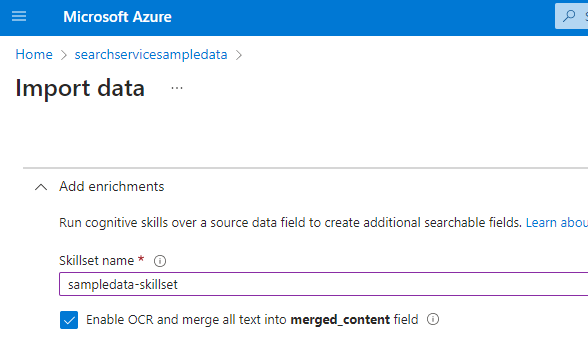
\includegraphics[scale=0.8]{images/Chapter4/enable_ocr.png}}
                \caption{Creating a skillset (\textit{sampledata-skillset}) and enabling \acs{OCR}}
                \label{enableocr}
            \end {figure}
        
            There was a list of Cognitive (both Text and Image) skills to choose from. Figure \ref{cogskillset} in Appendix shows a list of the available Cognitive skillset provided to choose from. The 'translate text' skill had 64 language choices in the drop-down menu\ref{translang}. The field names were editable to the user's choice (these names would be used while querying the dataset). A few of the cognitive skills from the list were selected for testing as seen in Figure \ref{selectedskillset}.
            \begin {figure}[h!h]
                \centering
                \adjustbox{frame}{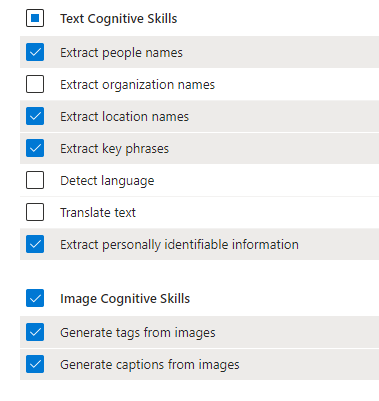
\includegraphics[scale=0.92]{images/Chapter4/selected_skillset.png}}
                \caption{Skillsets selected for testing}
                \label{selectedskillset}
            \end {figure}
            \item Third section was 'Save enrichments to a knowledge store'. In this section, the user could choose to save the enrichments (selected in the previous section) that would be extracted to a knowledge store, which could be used to visualize the enriched data in the form of tables, etc. Selected one of the projection options in this section too for testing.
        \end{enumerate} 
        \newpage
        \item Next step was 'Customize target index'. Created an index named \textit{sampledata-index}. An index was created with a list of default fields that appeared. The fields could be added/deleted to make an index required by the user. The user could also edit which fields needed to be Sortable\/Searchable and so on. The 'pii\_entities' field had sub-fields as seen in Figure \ref{piisubfields} where \textit{pii\_type} implies the category of \acs{PII} it belongs to; person, organization, phone number, etc. \cite{azurepiicategories} and \textit{pii\_score} signifies the potential of the information to identify an individual.
        \begin {figure}[h!h]
            \centering
            \adjustbox{frame}{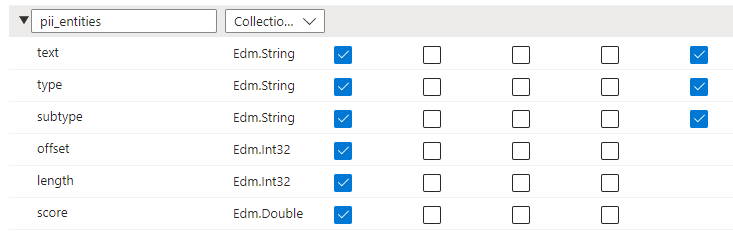
\includegraphics[scale=0.83]{images/Chapter4/pii_subfields.png}}
            \caption{Sub-fields in the pii\_entities field}
            \label{piisubfields}
        \end {figure}
        After making a few changes, the index looked as seen in Figures \ref{selectedfields1} and \ref{selectedfields2}.
        \begin {figure}[h!h]
            \centering
            \adjustbox{frame}{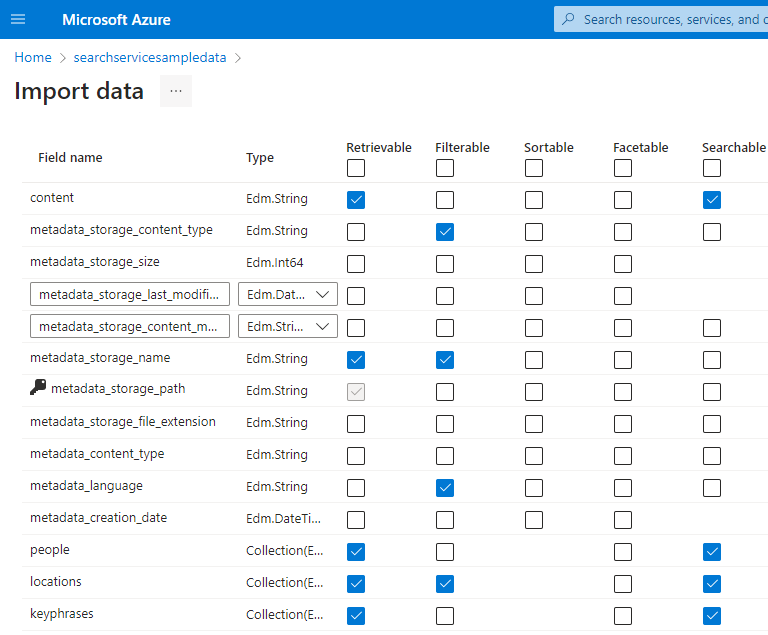
\includegraphics[scale=0.69]{images/Chapter4/selected_fields1.png}}
            \caption{Selected fields part-1}
            \label{selectedfields1}
        \end {figure}
        \begin {figure}[h!h]
            \centering
            \adjustbox{frame}{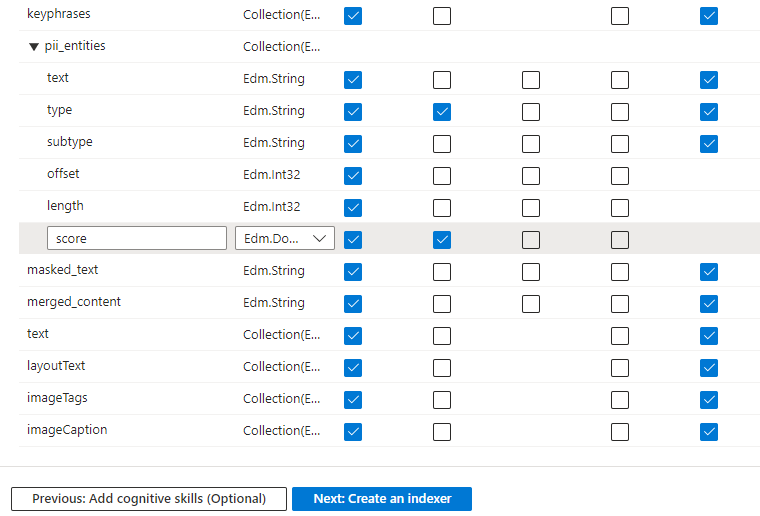
\includegraphics[scale=0.69]{images/Chapter4/selected_fields2.png}}
            \caption{Selected fields part-2}
            \label{selectedfields2}
        \end {figure}
        \clearpage
        \newpage
        \item Last step was 'Create an indexer'. Created an indexer named \textit{sampledata-indexer}. The user can also schedule how often an indexer should run in order to keep the index up to date.
    \end{itemize}
    \item Once the indexer was successfully created, queries were run on the index to view extracted results.
\end{itemize}
Below is a query and its result:
The query \\
\centerline{\texttt{'search=*\&$count=true\&$select=metadata\_storage\_name,pii\_entities'}}
gave results as a list of all document names (\textit{metadata\_storage\_name}) and all the \acs{PII} entities \textit{pii\_entities} within the document; specifying the text, type, score, etc. (all \acs{PII} sub-fields as seen in Figure \ref{piisubfields} above). Figure \ref{query1results} shows the results of the query. It shows the document name and a few of the \acs{PII} entities in the list. Text \textbf{'Institut für Parallele und Verteilte Systeme'} is identified as type \textit{Organisation} and \textbf{'Universitätsstraße 38'} as type \textit{Address}. 
\begin {figure}[h!h]
    \centering
    \adjustbox{frame}{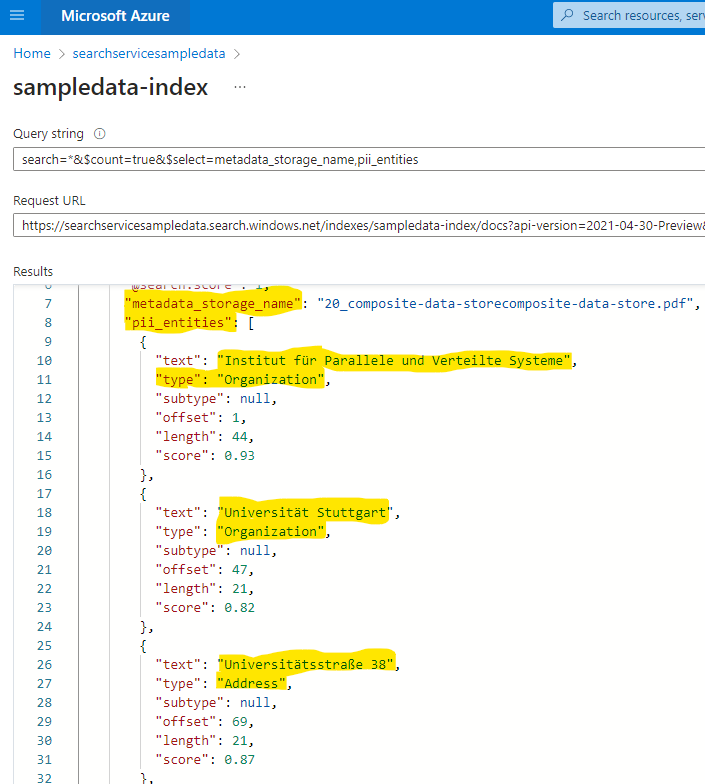
\includegraphics[scale=0.68]{images/Chapter4/pii_query1.png}}
    \caption{Results showing document name and list of pii\_entities in that document}
    \label{query1results}
\end {figure}

\newpage
A full list of the types and subtypes of the pii\_entities can be seen in \cite{azurepiicategories}. Figure \ref{query2results} is a snippet of a few more pii\_entities shown in the result where it has rightly identified '\textbf{Bernhard Mitschang} as type \textit{Person} and \textbf{'Betreuer'} is identified as type \textit{PersonType}. 
\begin {figure}[h!h]
    \centering
    \adjustbox{frame}{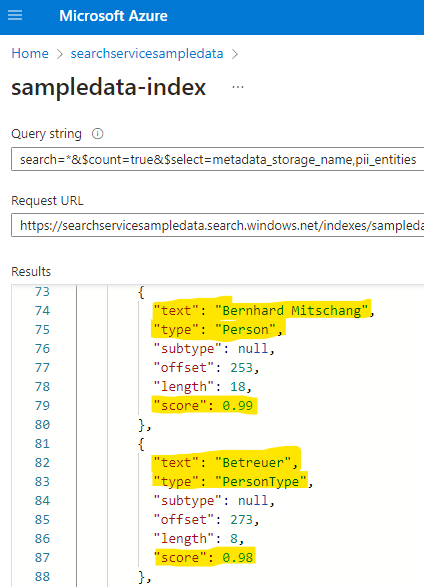
\includegraphics[scale=0.9]{images/Chapter4/pii_query2.png}}
    \caption{Results mentioning the sub-fields of some of the pii\_entities identified in one of the documents}
    \label{query2results}
\end {figure}
\\
Figures \ref{piisubtype} and \ref{datesubtype} show an example of identifying the 'subtype' field as well; this field was 'null' in previous snippets of the result. On the left, we see the field \textbf{June 20, 2011} and \textbf{November 24, 2011} being categorized as \textit{DateTime} type and accurately as \textit{Date} subtype as well. On the right, the text \textbf{2018} is categorized as \textit{DateTime} type and as \textit{DateRange} subtype as the month or date isn't specified, it is a whole range of time. \\
These were results from one query, user can write different queries in order to retrieve different sets of information needed by using the search, sort, and filter commands on the attributes selected while creating the index. Document with example queries explained in detail for reference to write queries \cite{azqueries}.
\begin {figure}[h!h]
    \centering
    \adjustbox{frame}{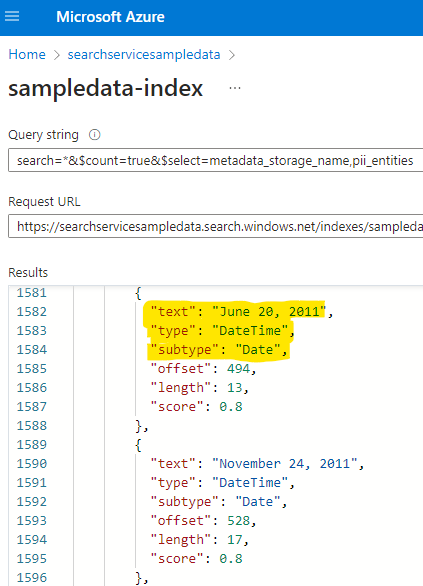
\includegraphics[scale=0.67]{images/Chapter4/pii_subtype.png}}
    \caption{Results snippet where the \textit{subtype} field is not null}
    \label{piisubtype}
\end {figure}
\begin {figure}[h!h]
    \centering
    \adjustbox{frame}{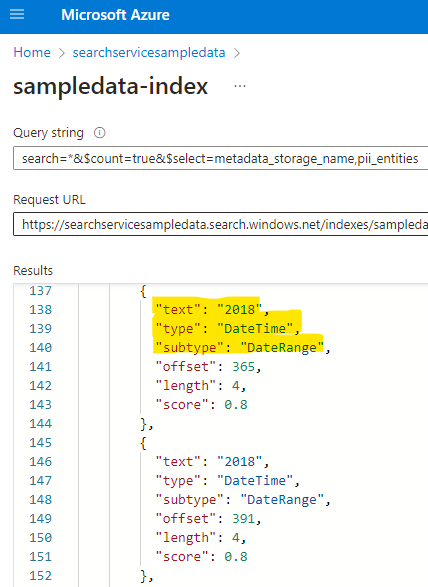
\includegraphics[scale=0.67]{images/Chapter4/date_subtype.png}}
    \caption{Results snippet where the \textit{subtype} field is not null}
    \label{datesubtype}
\end {figure}
\newpage
The implementation steps described so far was for 'Azure Cognitive Search Service'. Next, Figure \ref{createlangserv} shows the creation of \textbf{Azure Cognitive Services for Language} resource. It had default features like sentiment analysis, text summarization, named entity recognition, etc. pre-selected and provided two customizable features for the user to choose if needed. The second customizable feature was selected during the creation of this language service named \textit{cogservicelang}.
\begin {figure}[h!h]
    \centering
    \adjustbox{frame}{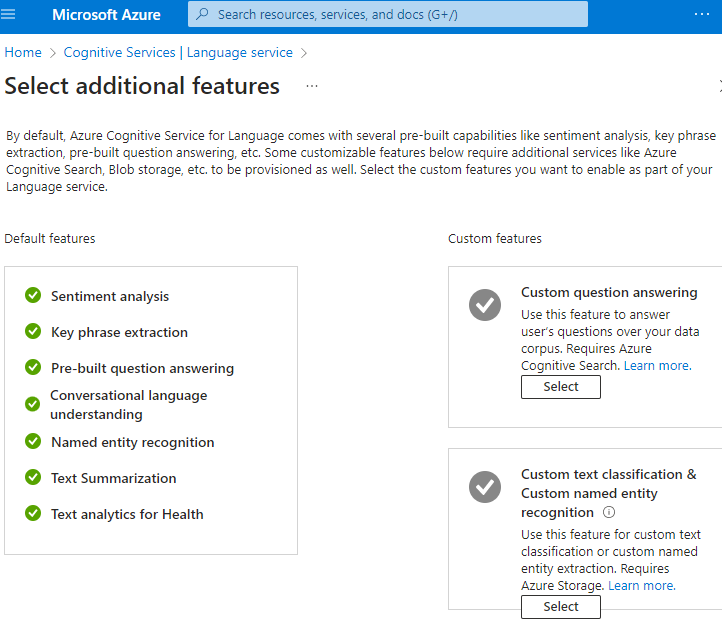
\includegraphics[scale=0.78]{images/Chapter4/create_lang_service.png}}
    \caption{Snippet of selection of a custom text classification and custom \acs{NER} features}
    \label{createlangserv}
\end {figure}

The author was unable to find any generic tutorials on how to use 'Azure Cognitive Services for Language' in the Microsoft Learn portal. There were however a few videos on specific aspects like exclusively for text classification or for Virtual Agent Bot. After creating the language service (\textit{cogservicelang}) and going to the resource overview, there was a link to Language studio \cite{azlangstudio} where the user could try all the default features listed in Figure \ref{createlangserv}. There were a total of six features available for the user to try out in the 'Extract Information' section.

Tried the features mentioned in evaluation matrix \ref{section:matrix}. Testing of these features for language service was only possible on a few of the sample text options provided on the site for tryout.
The detailed snippets of trying out the first feature 'Extract PII' or '\acs{PII} detection' can be seen in Appendix \ref{piitryout}, \ref{sampletexts}, \ref{piires}, \ref{piiogtext}. \\
The detailed snippets of trying out the second feature 'Extract Named Entities' or '\acs{NER}' can be seen in Appendix \ref{nertryout}, \ref{nerres1}, \ref{nerres2}, \ref{sortfilternerres}, \ref{nerogtext}. \\
The additional snippets of trying out the third feature 'Sentiment Analysis' can be seen in Appendix \ref{enableopinion}, \ref{opinionres}. \\
The additional snippet of trying out the fourth feature 'Summarization' can be seen in Appendix \ref{summinput}. \\
The detailed snippets of trying the fifth feature 'Text Classification' can be seen in Appendix \ref{nertryout}, \ref{nerres1}, \ref{nerres2}, \ref{sortfilternerres}, \ref{nerogtext}.
\begin{itemize}
    \item \uline{\acs{PII} detection:} The input text for \acs{PII} extraction is seen in Figure \ref{piiinput}. The output of the same text after performing \acs{PII} extraction can be seen in Figure \ref{piioutput}. Note that this snippet was taken after enabling the option 'Hide PII', hence the texts identified as \acs{PII} have been obscured or masked.\\
     \begin {figure}[h!h]
        \centering
        \adjustbox{frame}{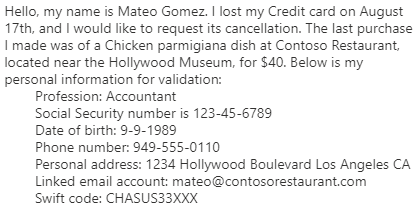
\includegraphics[scale=0.99]{images/Chapter4/pii_input.png}}
        \caption{Snippet of sample banking text used as input for \acs{PII} tryout}
        \label{piiinput}
    \end {figure}
    \begin {figure}[h!h]
        \centering
        \adjustbox{frame}{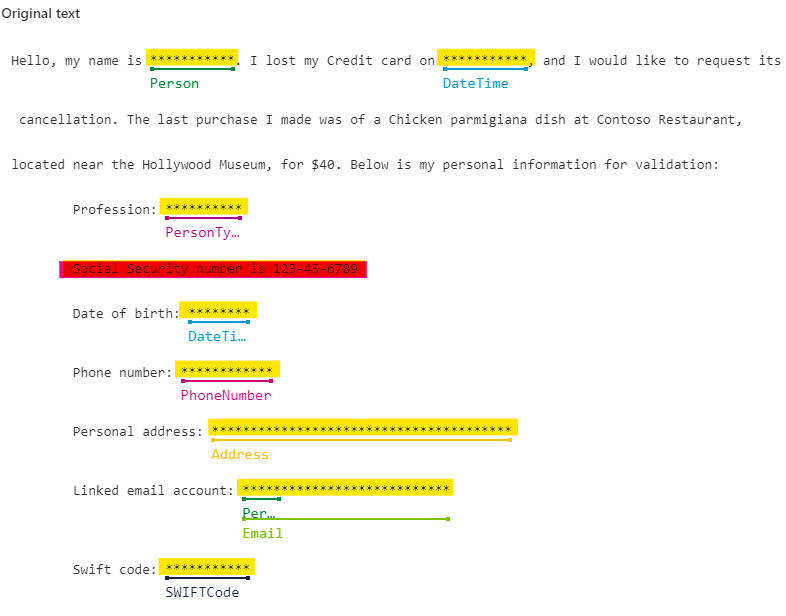
\includegraphics[scale=0.59]{images/Chapter4/pii_output.png}}
        \caption{Snippet showing the results of \acs{PII} extraction after obscuring the identified \acs{PII} entities on the sample banking text input}
        \label{piioutput}
    \end {figure}
    
    It is interesting to note in Figure \ref{piioutput} that the \textit{Social Security Number} '123-45-6789' (highlighted in red for reference) was not identified as an \acs{PII} entity. The sample text was semi-structured as it has the description of texts (Accountant, SSN, DOB, address) right in front of the actual information and hence raises the question of how well the \acs{PII} identification/extraction might work on unstructured data. 
    
    \item \uline{NER:} The input text for extraction of named entities is the same as the one used for extraction of \acs{PII}s (seen in Figure \ref{piiinput}). The output of the same text after performing \acs{NER} can be seen in Figure \ref{nerogtext1}. Note that this snippet as opposed to \ref{piiogtext} has all the named entities identified and categorized; not just the \acs{PII}s. Swift code which was recognized previously as \acs{PII} was not identified as an entity in \acs{NER} extraction.
    \begin {figure}[h!h]
        \centering
        \adjustbox{frame}{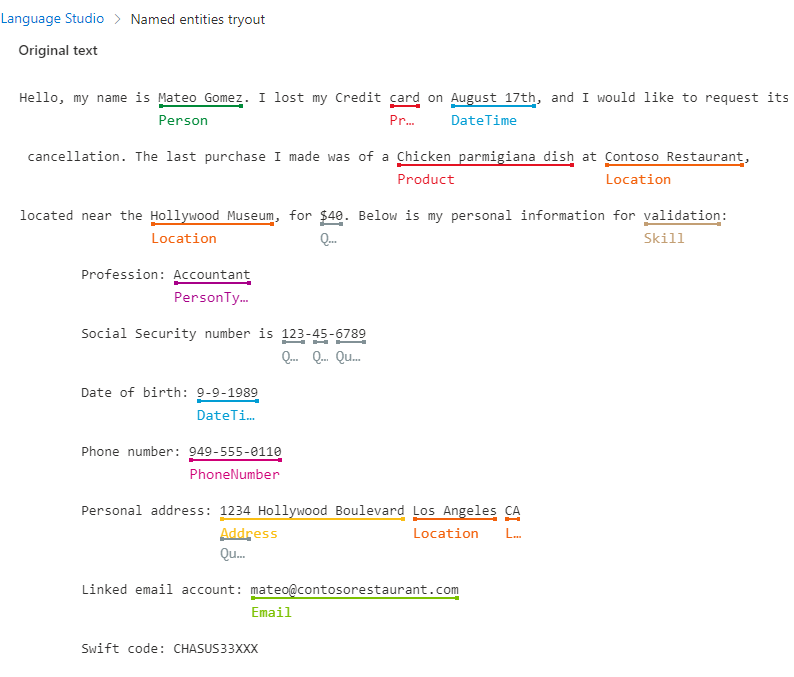
\includegraphics[scale=0.59]{images/Chapter4/ner_og_text.png}}
        \caption{Snippet showing the results of \acs{NER} on the sample banking text input}
        \label{nerogtext1}
    \end {figure}
    \newpage
    \item \uline{Sentiment Analysis:} The input text for Analyze Sentiment is seen in Figure \ref{sainput}. The results can be seen in Figure \ref{saoutput} which shows the sentiment of the document and drop-down options to view the sentiments of each statement in the document (left). When viewed for an individual statement, the sentiment and confidence for it are shown (right).
    \begin {figure}[h!h]
        \centering
        \adjustbox{frame}{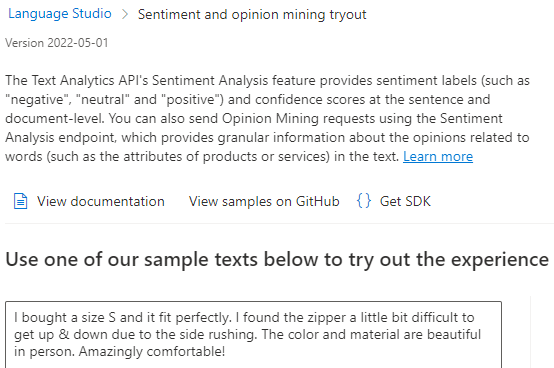
\includegraphics[scale=0.725]{images/Chapter4/sa_tryout.png}}
        \caption{Snippet of sample product review text used as input for Sentiment analysis}
        \label{sainput}
    \end {figure}
    \begin {figure}[h!h]
        \centering
        \adjustbox{frame}{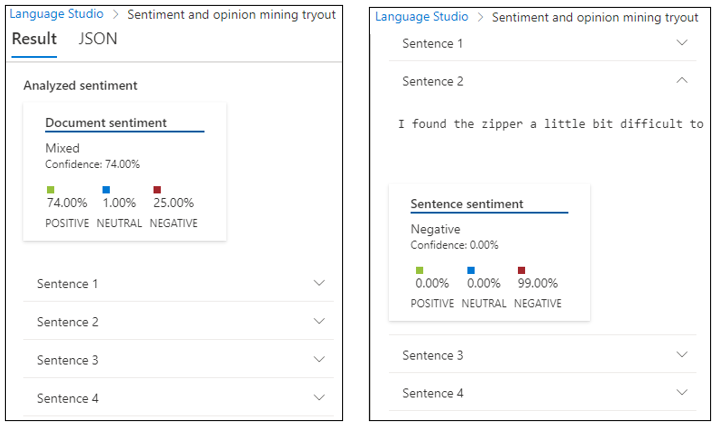
\includegraphics[scale=0.875]{images/Chapter4/sa_results.png}}
        \caption{Snippet showing the sentiment of the document and for one of the sentences}
        \label{saoutput}
    \end {figure}
    
    It is interesting to note in Figure \ref{saoutput} that the confidence is 0\% even though the sentence was rightly classified as 99\% Negative. For reference, Sentence-2 in this example was 'I found the zipper a little bit difficult to get up \& down due to the side rushing'. A snippet of Sentence-1 is shown in Appendix \ref{saconfilevel} for comparison of confidence levels (95\% for positive sentiment).
   
    \item \uline{Summarization:} The summarization feature could be used for documents as well as for conversations. It provided two types of summaries; Extractive summarization and Abstractive summarization. Users can choose to get both or either one of the summaries for their input. Similarly, it provides a few aspects of summarization when summarizing a conversation. The list of summary types for documents and different aspects possible while summarizing conversations is seen in Figure \ref{summzaspect}. The output of summarization can be seen in Figure \ref{summzresp} for summarizing the document and in Figure \ref{summzresp2} output for summarizing the conversation. The conversation input for summarization can be seen in Appendix \ref{summinput}.
    \begin {figure}[h!h]
        \centering
        \adjustbox{frame}{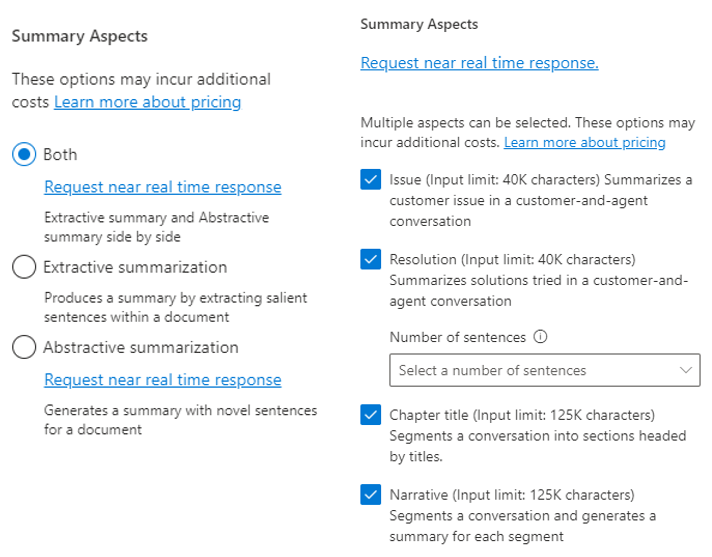
\includegraphics[width=0.95\textwidth]{images/Chapter4/summ_asp.png}}
        \caption{Snippet of options available for summarizing documents (left) and summarizing conversation (right)}
        \label{summzaspect}
    \end {figure}
    \begin {figure}[h!h]
        \centering
        \adjustbox{frame}{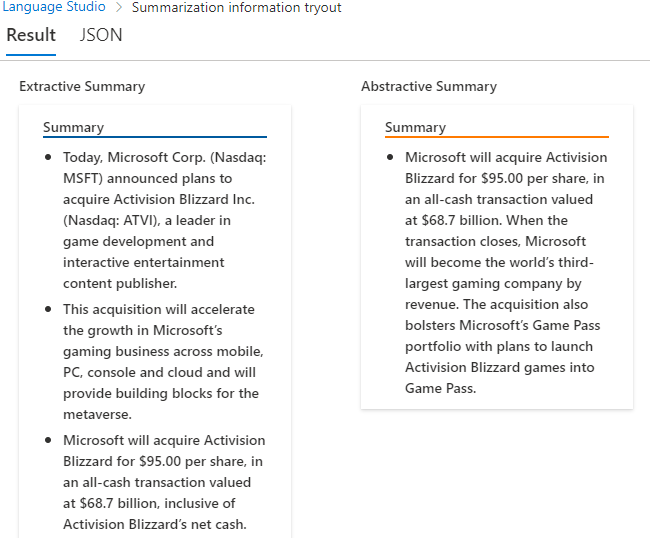
\includegraphics[scale=0.64]{images/Chapter4/summ_res.png}}
        \caption{Snippet of summary results for document displaying both Extractive Summary (left) and Abstractive Summary (right)}
        \label{summzresp}
    \end {figure}
    \begin {figure}[h!h]
        \centering
        \adjustbox{frame}{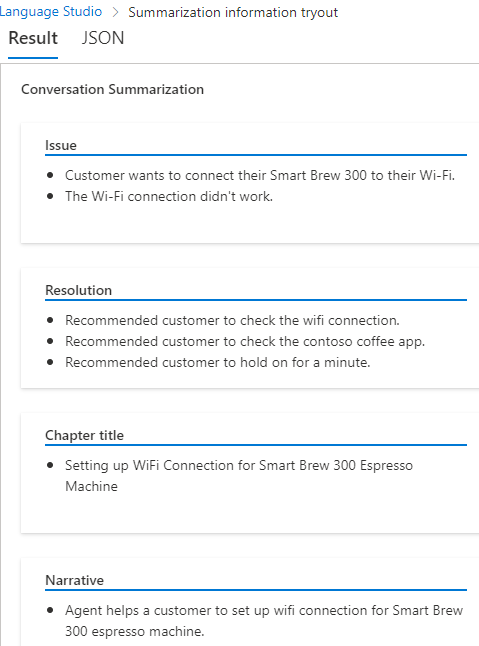
\includegraphics[scale=0.657]{images/Chapter4/summ_res2.png}}
        \caption{Snippet of summary results for conversation}
        \label{summzresp2}
    \end {figure}
    \clearpage
    \newpage
    \item \uline{Classification:} The custom text for Classification was supported for both single-label classification and multi-label classification. For instance, 
    
    1) In single-label classification, input (a document) would be classified into only one category/class. Example: Any input 'xxxxx' would only be classified as either 'health' or 'robotics'. \\
    2) In multi-label classification, an input could be categorized into more than one class. Example: Input 'xxxxx' could be classified into just the 'health' class or both 'health' and 'robotics' classes \cite{azcustomtextclassification}.
    
    For testing of this feature, there were no sample texts available like for the above four features. A new project for this feature had to be created. This was not possible even though the creation of a language service named \textit{cogservicelang} was done in the Azure portal as seen in Figure \ref{langres}. Further details and snippets showing the attempt to test the Text classification feature can be seen in Appendix \ref{textclass1}, \ref{textclass2}.
    \begin {figure}[h!h]
        \centering
        \adjustbox{frame}{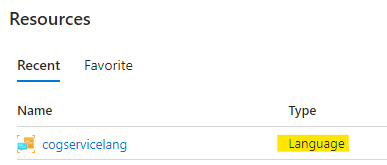
\includegraphics[scale=1]{images/Chapter4/lang_resource.png}}
        \caption{Snippet showing the created Language resource in Azure portal}
        \label{langres}
    \end {figure}
\end{itemize}
Testing these features with custom datasets was not possible in the Student subscription account used by the author. The three datasets described in \ref{section:dataset} were used in testing the 'Azure Cognitive Search service'. There was no option to test 'Azure Cognitive Services for Language' with them, because of the student subscription account limitations. Hence, testing of the Language service was only possible to the extent of the sample texts provided on the website. 

IBM also provided a live demo of IBM Watson's Natural Language Understanding \cite{ibmdemo}. Input to test the features was only possible in either of the three options: 1). Sample texts provided on the site, 2). Custom text (no option to upload a document, just writing/pasting paragraph of text) and 3).\acs{url} to a website page.
As there was an option to use custom text, tried the same input texts used to test Azure Cognitive Services for Language in order to be able to compare the results by both cloud service providers.
There was no option in the demo to test for \acs{PII} detection and summarization. 
\begin {figure}[h!h]
        \centering
        \adjustbox{frame}{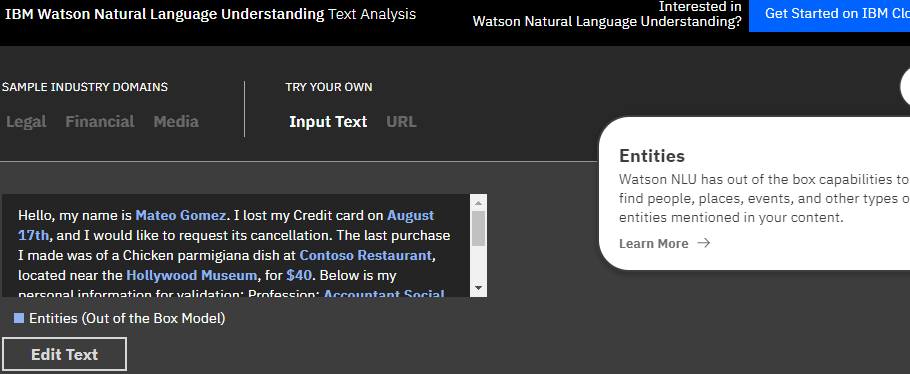
\includegraphics[scale=0.69]{images/Chapter4/ibm_entity_ip.png}}
        \caption{Snippet showing the demo website, entities extraction}
        \label{ibmnerip}
    \end {figure}
\begin {figure}[h!h]
        \centering
        \adjustbox{frame}{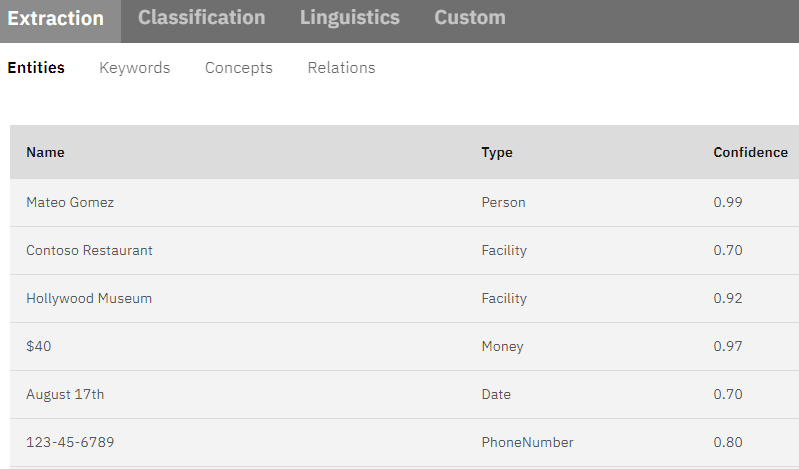
\includegraphics[scale=0.775]{images/Chapter4/ibm_entity_op1.png}}
        \caption{Snippet showing the list of entities extracted part-1}
        \label{ibmnerop1}
    \end {figure}
\newpage
Started with testing for extraction of entities. The input was the same as in the case of Azure (Figure \ref{piiinput}); the snippet is shown in Figure \ref{ibmnerip}. The output was obtained as a list of entities with their type and confidence level. The output list of entities is shown in Figures \ref{ibmnerop1}, \ref{ibmnerop2}, and \ref{ibmnerop3}. It extracted 14 entities as opposed to Azure, which extracted 19 entities. IBM identified 'Social Security' as an entity of type \textit{organization}. IBM also identified '33' which was part of the text 'swift code' as an entity of type \textit{number}. These were not identified in Azure. Azure did not identify the security number '123-45-6789', it instead identified '123', '45', and '6789' as 3 separate entities of type \textit{number}. IBM on the other hand identified '123-45-6789' as a phone number. But IBM did not identify a few entities like 'card' (type \textit{product}), 'Chicken parmigiana dish' (type \textit{product}), and 'validation' (type \textit{skill}) which were identified in Azure \ref{nerres1} \ref{nerres2}.
\begin {figure}[h!h]
        \centering
        \adjustbox{frame}{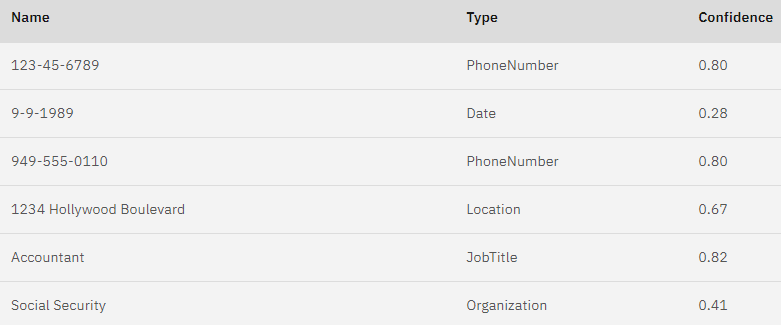
\includegraphics[scale=0.79]{images/Chapter4/ibm_entity_op2.png}}
        \caption{Snippet showing the list of entities extracted part-2}
        \label{ibmnerop2}
    \end {figure}
\begin {figure}[h!h]
        \centering
        \adjustbox{frame}{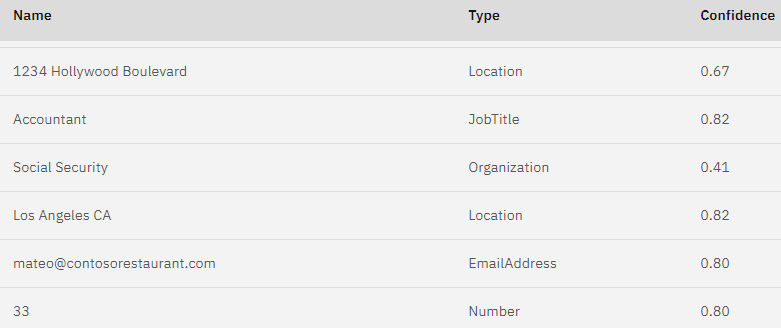
\includegraphics[scale=0.79]{images/Chapter4/ibm_entity_op3.png}}
        \caption{Snippet showing the list of entities extracted part-3}
        \label{ibmnerop3}
    \end {figure}

%\newpage  
After testing for entities, sentiment analysis was tested next. The input was the same text used to test the sentiment analysis feature in Azure \ref{sainput}. The input screen can be seen in Figure \ref{ibmsaip}. Confidence of Sentiment classification was only specified for classes identified, unlike Azure which had confidence levels mentioned for each of the sentiment classes (even if it was 0\%). Sentiment classification results of IBM \acs{NLU} can be seen in Figure \ref{ibmsaop}. The sentiment of the text was analyzed as Positive by both cloud service providers. There was a 4\% difference in their confidence levels. IBM had a confidence of 78\% for Positive sentiment classification whereas Azure had 74\% confidence for Positive (25\% Negative and 1\% Neutral). Azure provided sentiment analysis for each sentence in the input which was not provided in IBM. But IBM had sentiment scores for keywords (Figure \ref{ibmsaop}) that were not available in Azure.
\begin {figure}[h!h]
    \centering
    \adjustbox{frame}{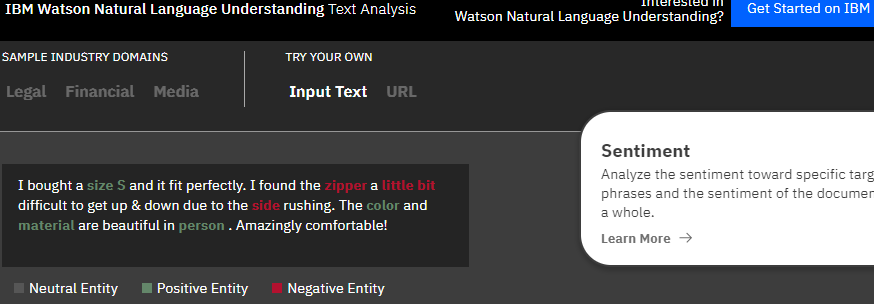
\includegraphics[scale=0.72]{images/Chapter4/ibm_sa_ip.png}}
    \caption{Snippet showing the sentiment analysis input}
    \label{ibmsaip}
\end {figure}
\begin {figure}[h!h]
    \centering
    \adjustbox{frame}{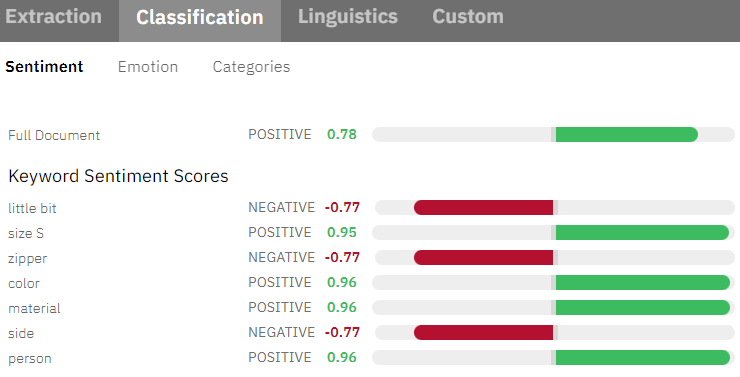
\includegraphics[scale=0.85]{images/Chapter4/ibm_sa_op.png}}
    \caption{Snippet showing the sentiment analysis results}
    \label{ibmsaop}
\end {figure}

In Google Cloud Documentation \cite{gcdocs2}, there was a list of features along with a description as shown in Figure \ref{gcfeatures}. As there was no free access, could not try the features with chosen datasets as in the case of Azure. Google had small lab sessions to give a glimpse of the features of their services. The lab session was in the form of tutorials, came with a set of instructions, and very limited access to the features. In this lab tutorial \cite{gcqwiklab}, it was possible to test entity recognition, sentiment analysis, and other features. A snippet of testing sentiment analysis is shown in Figure \ref{gcsenti}. Results for the 'analyze entities' feature for the statement \textit{'Michelangelo Caravaggio, Italian painter, is known for 'The Calling of Saint Matthew''} is shown in Figure \ref{gcner}.
\begin {figure}[h!h]
    \centering
    \adjustbox{frame}{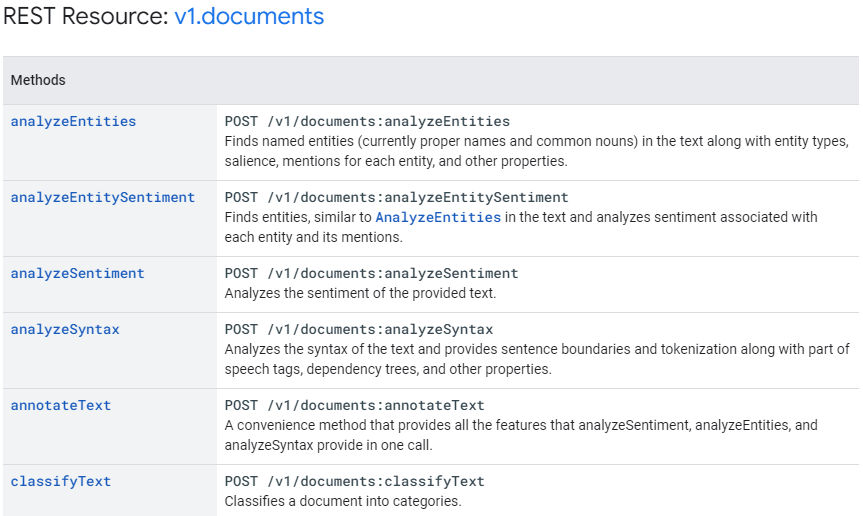
\includegraphics[scale=0.727]{images/Chapter4/gc_features.png}}
    \caption{Snippet showing the features available in Google Cloud Natural Language}
    \label{gcfeatures}
\end {figure}
\begin {figure}[h!h]
    \centering
    \adjustbox{frame}{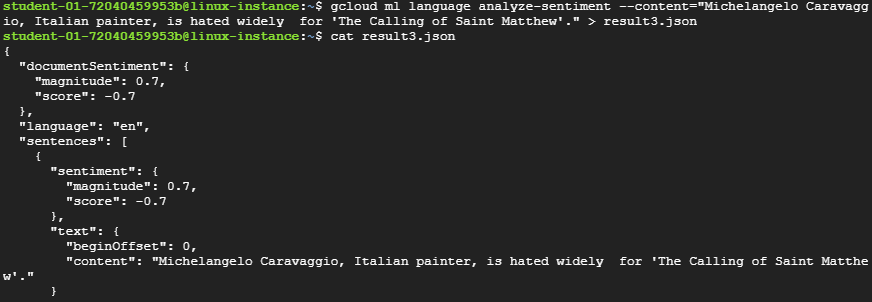
\includegraphics[scale=0.715]{images/Chapter4/gc_senti_analysis.png}}
    \caption{Snippet showing the sentiment analysis in qwiklab session}
    \label{gcsenti}
\end {figure}
\begin {figure}[h!h]
    \centering
    \adjustbox{frame}{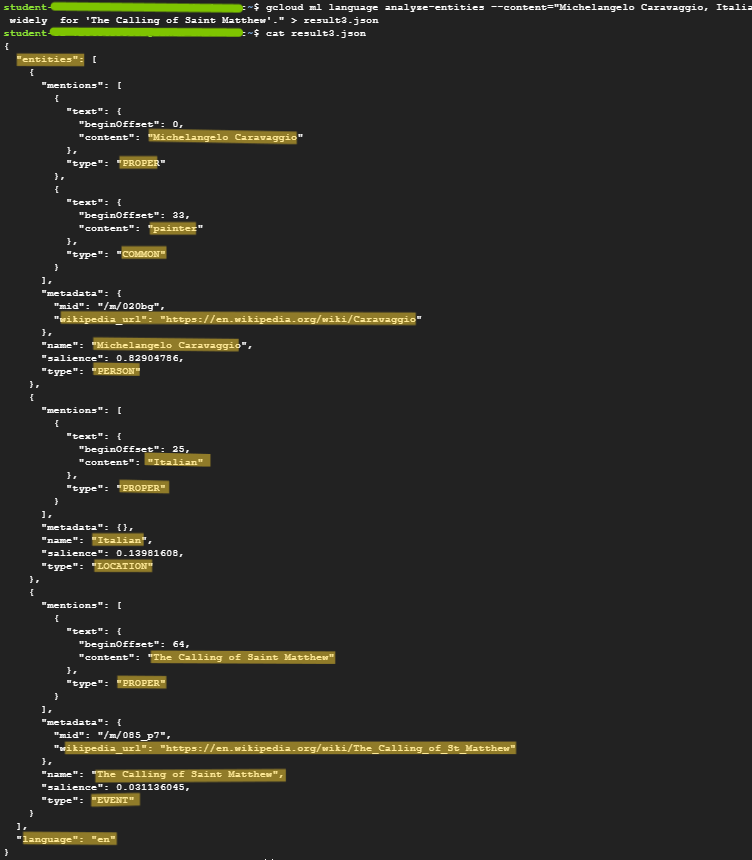
\includegraphics[height=18cm, width=1\textwidth]{images/Appendix_images/gc_ner_highlught.png}}
    \caption{Snippet showing the results for 'analyze-entities'}
    \label{gcner}
\end {figure}